\documentclass[10pt]{article}
\usepackage[utf8]{inputenc}
\usepackage{amsmath}
\usepackage{amssymb}
\usepackage{graphicx}
\usepackage{hyperref}
\usepackage{menukeys}
\usepackage{nameref}
\usepackage{listings}
\title{openAPE}
\author{Stephan Unfried}
\date{\today} 
\begin{document}
\maketitle
\newpage
\tableofcontents
\newpage
\section{Introduction}
\section{project structure}
\subsection{Modules}
The project consists of tree parts, represented in tree maven modules. For details of the associations see figure \ref{fig:moduleuml}.
\begin{figure}[b]
\centering
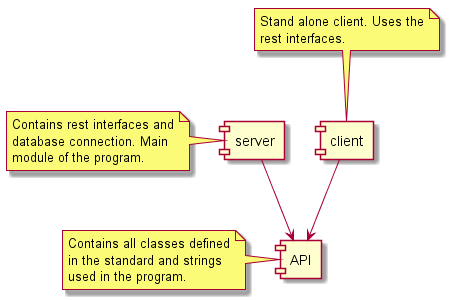
\includegraphics[width=0.8\textwidth]{uml/modulesuml.png}
\caption{module diagram.}
\label{fig:moduleuml}
\end{figure}
\subsection{API}
API contains classes and class structure used by the application server and clients who want to communicate with it. The classes contained in the API module represent the objects stored in the application. For clients it is important to uphold the class structure for the server to recognize those objects. For the structure of the module see figure \ref{fig:apiuml}.
\begin{figure}[b]
\centering
\makebox[\textwidth][c]{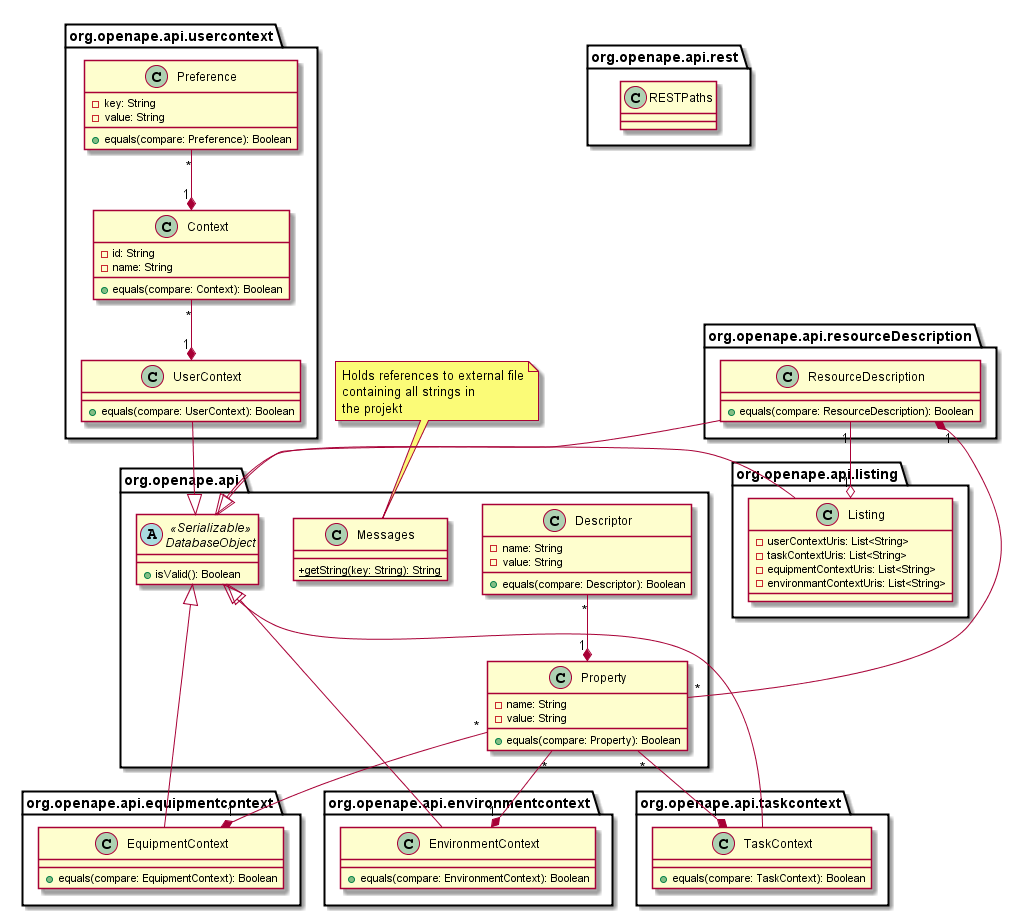
\includegraphics[width=1.4\textwidth]{uml/apiuml.png}}
\caption{API module structure diagram.}
\label{fig:apiuml}
\end{figure}
\subsection{Server}
The Server module is the main module of the application. It contains the web application used to up- and download contents. It provides an rest interface for access and uses a mongoDB and the file system to store data. The \emph{mongoDB} access can be configured in \directory{classes/config/mongo.properties}. For using the rest paths see the \emph{ISO-IEC\_CD\_24752-8} Standard. For the module structure see figure \ref{fig:serveruml}.
\begin{figure}[b]
\centering
\makebox[\textwidth][c]{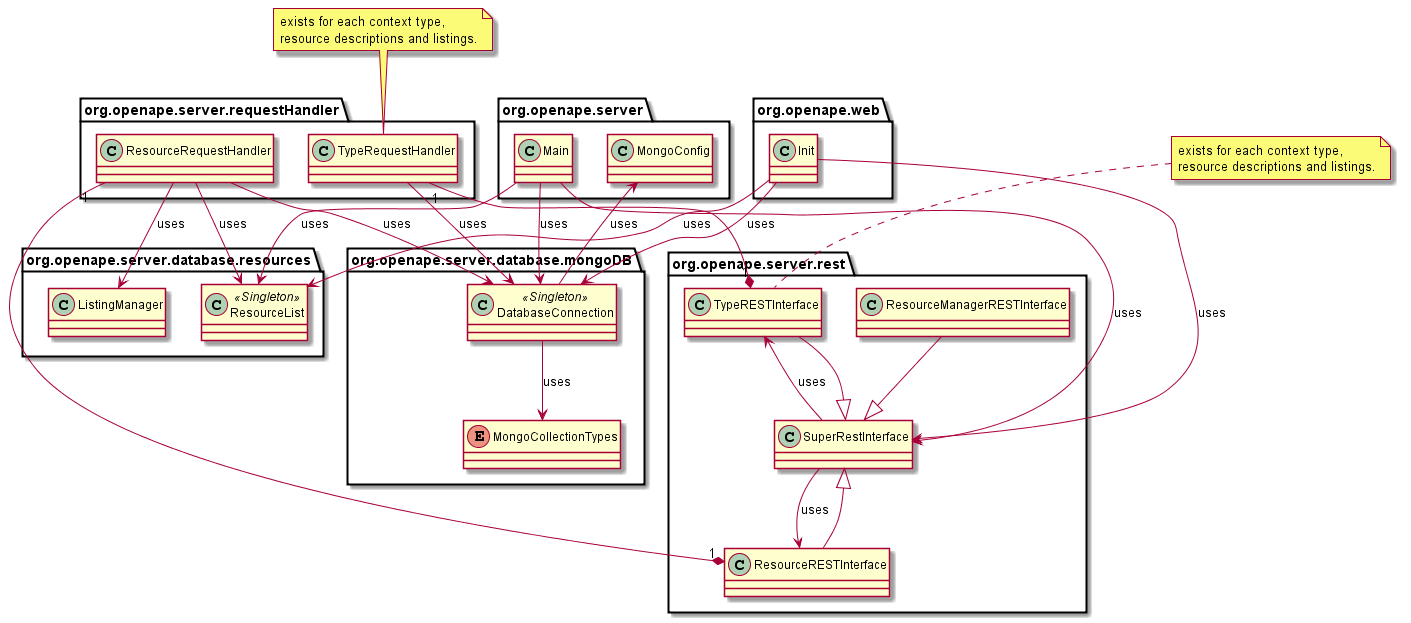
\includegraphics[width=1.5\textwidth]{uml/serveruml.png}}
\caption{Server module structure diagram.}
\label{fig:serveruml}
\end{figure}
\subsection{Client}
The Client is a sand alone module that uses the rest interface of the server to communicate with it. It can be replaced by any application capable of generating rest requests and processing the result.
\section{Get started with the project}
\paragraph{Remark} This section shows how to set up a development environment to work with the project. To see how to deploy the application for use please skip forward to section \nameref{sec:setupapp}.
\subsection{Git repository}
To use the repository used for this project you need a \emph{Github} account and an application capable of running git commands.
\paragraph{Github account} To create an account visit the \href{https://github.com/}{Github homepage}.
\paragraph{Git application} On \emph{Linux} systems use your package installer to install a current git package. You can use the normal shell to run git commands. On \emph{Windows} you can use the \emph{Github} application from their \href{https://github.com/}{homepage} and the build in git shell to run git commands.
\paragraph{Git repository} To clone the repository use your console, which is able to use git commands, and navigate to the location where it should be cloned to. Then use \texttt{git clone https://github.com/REMEXLabs/OpenAPE}. You will be asked so sign in with your \emph{Github} credentials.
\subsection{Eclipse}
The project is developed in \emph{Eclipse} and so here is described how to use it. But any IDE can be used that provides \emph{Maven} support.
\paragraph{Install Eclipse} The current version of \emph{Eclipse} can be found on their \href{https://eclipse.org/downloads/}{download page}.
\paragraph{Install Java} To develop this project with \emph{Eclipse} you need a current \emph{Java Development Kit}. Use the download button under \emph{JDK} \href{http://www.oracle.com/technetwork/java/javase/downloads/index.html}{here} to get the current version.
\paragraph{Import project} It is recommended not to use the project folder as workspace for \emph{Eclipse} but to import the project. To do so start \emph{Eclipse} and navigate $File \rightarrow Import... \rightarrow Maven \rightarrow \text{\emph{Existing Maven Projects}} \rightarrow Next \rightarrow Browse... \rightarrow \text{browse the folder OpenAPE/openAPE} \rightarrow -> Finish$. Now you should have the main project plus the modules \emph{API} \emph{client} and \emph{server} in your navigation.
\paragraph{Ensure the right Java version is used} The project will not work correctly if \emph{Eclipse} doesn't use the previously installed \emph{Java JDK} but a \emph{Java RE}. To change the used \emph{Java version} mark a module and navigate $Project \rightarrow Properties \rightarrow \text{emph{Java Build Path}} \rightarrow Libraries \rightarrow \text{mark the used system library} \rightarrow Edit... \rightarrow \text{emph{Execution environment}} \rightarrow \text{Choose a Java 1.8 JDK or newer from the list and klick finish. If none is available navigate \emph{Installed JREs…}} \rightarrow Search... \rightarrow  \text{Choose the installation path of the previously installed Java JDK. It should now be available in the execution environment list}.$ Repeat this process for each module containing source code.
\subsection{Maven} \emph{Maven} is a build automation tool used to compile the project and create the deployable \emph{war file}. Next is the order in which \emph{Maven} commands are used to create the \emph{war}. After importing the project this should be done once to update the projects \emph{build path} and get rid of errors regarding it. 
\paragraph{Maven deployment commands} $\text{Right click on the main project} \rightarrow Maven \rightarrow \text{\emph{Update Project...}}$

$\text{Right click on the main project} \rightarrow \text{\emph{Run As}} \rightarrow \text{\emph{Maven clean}}$

$\text{Right click on the main project} \rightarrow \text{\emph{Run As}} \rightarrow \text{\emph{Maven install}}$

After each command wait for the IDE to finish. After the last command there should be a deployable \emph{war} file in \directory{server/target}.
\section{Set up application}
\label{sec:setupapp}
The application needs an installed and running \emph{mongoDB} to work. So first it is described how to set up that. The application itself can run on any web server capable of deploying a \emph{war} file. Here is described how to deploy it onto a tomcat server.
\subsection{Set up MonoDB}
\subsection{Set up tomcat server}
\end{document}
